\documentclass{article}

\usepackage{neurips_2024}

\usepackage[utf8]{inputenc}
\usepackage[T1]{fontenc}
\usepackage{hyperref}
\usepackage{url}
\usepackage{booktabs}
\usepackage{amsfonts}
\usepackage{amsmath}
\usepackage{amssymb}
\usepackage{amsthm}
\usepackage{nicefrac}
\usepackage{microtype}
\usepackage{xcolor}
\usepackage{algorithm}
\usepackage{algorithmic}
\usepackage{graphicx}
\usepackage{multirow}
\usepackage{subcaption}
\usepackage{bm}
\usepackage{enumitem}
\usepackage{wrapfig}
\usepackage{thmtools}

\newtheorem{theorem}{Theorem}
\newtheorem{lemma}[theorem]{Lemma}
\newtheorem{proposition}[theorem]{Proposition}
\newtheorem{corollary}[theorem]{Corollary}
\newtheorem{remark}{Remark}
\newtheorem{definition}{Definition}
\newtheorem{assumption}{Assumption}

\newcommand{\erank}{\mathrm{erank}}
\newcommand{\tr}{\mathrm{tr}}
\newcommand{\diag}{\mathrm{diag}}
\newcommand{\RR}{\mathbb{R}}
\newcommand{\EE}{\mathbb{E}}
\newcommand{\cL}{\mathcal{L}}
\newcommand{\cT}{\mathcal{T}}
\newcommand{\cW}{\mathcal{W}}
\newcommand{\cH}{\mathcal{H}}
\newcommand{\cS}{\mathcal{S}}
\newcommand{\cN}{\mathcal{N}}
\newcommand{\cO}{\mathcal{O}}

\title{Can the Optimizer Prevent Loss of Plasticity? \\ Second-Order Methods Meet Spectral Diversity Preservation}

\author{%
  Anonymous Author(s) \\
  \texttt{anonymous@institution.edu}
}

\begin{document}

\maketitle

\begin{abstract}
Neural networks trained continually on sequences of tasks gradually lose the ability to learn new information---a phenomenon termed \emph{loss of plasticity} (LoP). While existing solutions predominantly target architecture or explicit regularization, the role of the \emph{optimizer itself} remains underexplored. We ask: \textbf{can second-order optimizers---which exploit curvature information---inherently mitigate LoP?} Through a systematic investigation combining theory and extensive experiments, we uncover a nuanced answer governed by two factors: \emph{network depth} and \emph{normalization structure}. In deep networks with batch normalization, second-order methods automatically maintain plasticity (near-zero dormant neurons, high stable rank $\|W\|_F^2/\sigma_{\max}^2$) by exploiting the well-conditioned Hessian spectrum that BN provides---yet they overfit due to convergence to sharp minima. In shallow networks without BN, outlier Hessian eigenvalues degrade preconditioning quality, causing second-order methods to \emph{lose} plasticity despite retaining generalization capacity. We formalize these observations through a theoretical framework linking Hessian spectral conditioning to effective rank preservation under preconditioned updates. To bridge the gap, we propose \textbf{Spectral Diversity Preservation (SDP)}, a geometric-mean interpolation on weight singular values applied at task boundaries:
\[
  \sigma'_i = \bar{\sigma}^\gamma \cdot \sigma_i^{1-\gamma},\quad \bar{\sigma} = \tfrac{1}{r}\textstyle\sum_j \sigma_j,\quad \gamma\in(0,1].
\]
SDP acts as a \emph{spectral analog of batch normalization}---compressing the eigenspectrum without architectural constraints---enabling second-order methods to maintain plasticity in BN-absent networks and preventing sharp-minima overfitting in deep networks. Experiments across three second-order optimizers (AdaHessian, SophiaH, SASSHA), three benchmarks (Incremental CIFAR-100, Permuted MNIST, continual RL), and comparisons with first-order baselines demonstrate that SDP combined with second-order optimization consistently achieves the lowest dormant neuron ratios, highest stable ranks, and best test accuracy.
\end{abstract}

%=============================================================================
\section{Introduction}
\label{sec:intro}
%=============================================================================

Neural networks excel in stationary settings, yet suffer a troubling degradation when the data distribution shifts over time. In continual learning~\citep{zenke2017continual}, reinforcement learning with non-stationary environments~\citep{schulman2017proximal, abbas2023loss}, and online adaptation, networks gradually lose their capacity to learn new information---a phenomenon termed \emph{loss of plasticity} (LoP)~\citep{lyle2023understanding, dohare2024loss}. Unlike catastrophic forgetting, which concerns the erasure of prior knowledge, LoP reflects a fundamental erosion of the network's \emph{learning capacity itself}: eventually, a continually trained deep network performs no better than a shallow network~\citep{dohare2024loss}.

The symptoms of LoP are well-characterized and interrelated. The fraction of \emph{dormant neurons}---units producing near-zero activations---increases over training~\citep{sokar2023dormant}. The \emph{stable rank} of weight matrices and feature representations collapses, reducing expressive capacity~\citep{he2024spectral}. Weight magnitudes grow unboundedly, saturating activation functions. The generalization gap widens. Recent theoretical work has deepened our understanding of \emph{why} these symptoms arise. \citet{lewandowski2024curvature} demonstrated that the loss of meaningful curvature directions in the Hessian spectrum---\emph{Hessian spectral collapse}---precedes and predicts LoP, rendering gradient-based optimization ineffective for new tasks. Most critically, \citet{joudaki2026barriers} provided a dynamical-systems formalization, proving that LoP arises from the entrapment of gradient dynamics within \emph{invariant sub-manifolds} of parameter space---frozen-unit manifolds from activation saturation and cloned-unit manifolds from representational redundancy---and that the very mechanisms promoting generalization in static settings (low-rank compression, geometric simplification) actively steer networks into these LoP manifolds.

\paragraph{Existing solutions and their limitations.} Current approaches to LoP predominantly modify the architecture or add explicit regularization atop standard first-order optimizers. Continual backpropagation~\citep{dohare2024loss} randomly reinitializes dormant neurons, injecting diversity through a non-gradient mechanism. Regenerative regularization~\citep{kumar2023maintaining} penalizes deviation from initial weights. \citet{lyle2025disentangling} showed that a combination of layer normalization and weight decay mitigates multiple independent causes of plasticity loss simultaneously. Self-normalized resets~\citep{lewandowski2025snr} adaptively detect and reset neurons with zero firing rates. Spectral regularization constrains the maximum singular value of weight matrices~\citep{miyato2018spectral}. However, all these methods operate \emph{atop first-order optimizers} (SGD, Adam), leaving a fundamental question unaddressed.

\paragraph{Our research question.} \textbf{Can the optimizer itself---through its use of curvature information---mitigate loss of plasticity?} This question is motivated by a convergence of theoretical insights:
\begin{enumerate}[leftmargin=*,nosep]
    \item \citet{lewandowski2024curvature}: Loss of curvature information is a root cause of LoP $\Rightarrow$ optimizers maintaining curvature awareness may resist it.
    \item \citet{gurari2018gradient}: Gradient descent operates in a tiny subspace of the top Hessian eigenvectors $\Rightarrow$ first-order updates are inherently low-rank, driving rank collapse.
    \item \citet{joudaki2026barriers}: First-order gradient dynamics are trapped in LoP manifolds due to the vanishing of transverse gradient components $\Rightarrow$ second-order methods, whose update geometry differs fundamentally, may escape these manifolds.
    \item \citet{ghorbani2019investigation}: Batch normalization suppresses outlier Hessian eigenvalues $\Rightarrow$ the Hessian spectral structure mediates whether second-order methods can leverage curvature effectively.
\end{enumerate}

\paragraph{Key observations.} Through systematic experiments across network depths and architectures, we observe a striking depth-dependent dichotomy:
\begin{itemize}[leftmargin=*,nosep]
    \item \textbf{Shallow networks without BatchNorm} (e.g., 3-layer MLP on Permuted MNIST): Second-order methods \emph{cannot} maintain plasticity---feature rank collapses dramatically and dormant neurons proliferate---but they \emph{can} generalize effectively on the tasks they do learn. The mechanism: without BN, large outlier eigenvalues in the Hessian spectrum~\citep{ghorbani2019investigation} degrade the quality of second-order preconditioning, effectively reducing it to a poorly-scaled first-order update.
    \item \textbf{Deeper networks with BatchNorm} (e.g., ResNet-18 on CIFAR-100): Second-order optimizers \emph{automatically} maintain plasticity (dormant neuron ratio $\approx 0$, stable rank remains high), but suffer from \emph{overfitting} due to convergence to sharp minima~\citep{shin2025sassha}, yielding poor test accuracy ($< 0.70$ on later tasks). BN smooths the Hessian spectrum, enabling effective preconditioning; but second-order methods' rapid convergence to precise (sharp) solutions prevents generalization.
\end{itemize}

\paragraph{Contributions.} We make four contributions:
\begin{enumerate}[leftmargin=*,nosep]
    \item \textbf{Theoretical framework} (Section~\ref{sec:theory}): We prove that second-order updates preserve a lower bound on the effective rank of weight matrices (Theorem~\ref{thm:rank_preservation}), contingent on the Hessian condition number. We provide a formal definition of $\kappa(G)$ for rectangular gradient matrices and a complete proof of the effective-rank bound. We formalize how BatchNorm mediates this effect through Hessian spectral smoothing, and clarify when and why first-order methods do \emph{not} benefit equally from BN (Proposition~\ref{prop:first_order_immune}).

    \item \textbf{Spectral Diversity Preservation (SDP)} (Section~\ref{sec:method}): A geometric mean interpolation on weight singular values---$\sigma'_i = \bar{\sigma}^\gamma \cdot \sigma_i^{1-\gamma}$---applied at task boundaries. SDP provably reduces $\kappa(W)$ by exponent $(1-\gamma)$ while preserving singular subspaces.

    \item \textbf{SDP as spectral BatchNorm} (Section~\ref{sec:analysis}): We establish that SDP fulfills an analogous role to BN for the weight spectrum: suppressing outlier singular values and preventing the condition number explosion that undermines second-order preconditioning in BN-absent architectures, while also preventing sharp-minima convergence in deep networks.

    \item \textbf{Extensive experiments} (Section~\ref{sec:experiments}): Three second-order optimizers $\times$ $\{$SDP, noSDP$\}$ across three benchmarks with first-order baselines, demonstrating consistent synergy. We include ablations isolating the contribution of optimizer state reset from SDP, report standard continual-learning metrics (average accuracy, backward transfer, forgetting), and detail SVD implementation for convolutional layers.
\end{enumerate}

%=============================================================================
\section{Background and related work}
\label{sec:background}
%=============================================================================

\subsection{Loss of plasticity in continual learning}

\textbf{Definition.} Following \citet{lyle2023understanding}, plasticity is the ability of a network to minimize loss on newly sampled objectives. A network \emph{loses plasticity} when its performance on new tasks degrades relative to a freshly initialized network, even with full access to new task data.

\textbf{Mechanistic understanding.} Multiple interacting mechanisms drive LoP. \emph{Hessian spectral collapse}~\citep{lewandowski2024curvature, he2024spectral}: meaningful curvature directions vanish at new-task initialization, rendering gradient descent ineffective. \emph{Feature rank collapse}~\citep{he2024spectral, xu2026forgetting}: the stable rank of intermediate representations decreases, reducing expressive capacity. \emph{Dormant neurons}~\citep{sokar2023dormant}: an increasing fraction of neurons produce near-zero activations, shrinking the effective network width. \emph{Weight magnitude growth}: unbounded parameter growth saturates activations. \citet{lyle2025disentangling} showed these mechanisms are partially independent---intervening on any single cause is insufficient, but intervening on multiple simultaneously is effective.

\textbf{Dynamical systems perspective.} \citet{joudaki2026barriers} provided the deepest theoretical treatment to date, formalizing LoP through dynamical systems theory. They identified two classes of \emph{invariant sub-manifolds} that trap gradient dynamics: \emph{frozen-unit manifolds} (from activation saturation, where units become unresponsive to gradient signals) and \emph{cloned-unit manifolds} (from representational redundancy, where multiple units compute identical functions). A fundamental tension emerges: the low-rank compression and geometric simplification that promote generalization in static settings---mechanisms related to neural collapse~\citep{papyan2020prevalence}---actively steer networks into these LoP manifolds. Crucially, they noted that second-order methods exhibit different dynamics on these manifolds because their update direction $P^{-1}\nabla\cL$ is not confined to the gradient subspace.

\textbf{Prior solutions.} Continual backpropagation~\citep{dohare2024loss} reinitializes low-utility neurons, demonstrating that a random non-gradient component is necessary for sustained plasticity. Self-normalized resets~\citep{lewandowski2025snr} detect and reset dormant neurons adaptively. Layer normalization + weight decay~\citep{lyle2025disentangling} address multiple mechanisms simultaneously. Curvature-aware replay~\citep{urettini2025ocar} uses Kronecker-factored Fisher information as a preconditioner in experience replay. Quasi-Newton continual learning~\citep{kong2025csqn} leverages quasi-Newton Hessian approximations for better parameter importance estimation. Elastic Weight Consolidation (EWC)~\citep{kirkpatrick2017ewc} uses Fisher information as a regularizer to prevent catastrophic forgetting but does not use curvature information in the update step itself. All prior plasticity-preservation methods operate with first-order optimizers or use curvature information only for regularization, not for the optimization update.

\subsection{Second-order optimization}

Second-order methods precondition gradient updates with curvature information:

\begin{definition}[Preconditioned update]
A second-order optimizer computes $\Delta \theta = -\eta P^{-1} \nabla_\theta \cL$, where $P \approx H = \nabla^2_\theta \cL$ is a positive-definite preconditioner.
\end{definition}

This preconditioning \emph{whitens} the gradient: directions of high curvature receive smaller steps, directions of low curvature receive larger steps, producing more isotropic updates than raw gradient descent. Table~\ref{tab:optimizers} summarizes the optimizers we study.

\begin{table}[t]
\caption{Second-order optimizers studied, distinguished by their Hessian approximation and generalization strategy.}
\label{tab:optimizers}
\centering
\small
\begin{tabular}{@{}lllll@{}}
\toprule
\textbf{Optimizer} & \textbf{Hessian Approx.} & \textbf{Key Property} & \textbf{Order} & \textbf{Reference} \\
\midrule
AdaHessian & Hutchinson diagonal & Per-param adaptive step & 2nd & \citet{yao2021adahessian} \\
SophiaH & Hutchinson + clipping & Element-wise clip, sparse update & 2nd & \citet{liu2023sophia} \\
SASSHA & SAM + Hutchinson & Sharpness + stable 2nd-order & 2nd & \citet{shin2025sassha} \\
\bottomrule
\end{tabular}
\end{table}

A critical finding from \citet{shin2025sassha} is that standard second-order methods tend to converge to \emph{sharper minima} than first-order methods, yielding worse generalization. SASSHA addresses this by integrating sharpness-aware minimization into the second-order framework. This observation is central to our analysis: maintaining plasticity (high rank, few dormant neurons) is necessary but not sufficient---the optimizer must also find flat minima for good generalization on new tasks.

\subsection{Related curvature-based continual learning methods}

\textbf{Natural-gradient and K-FAC methods.} Several continual learning approaches use curvature information differently from our work. EWC~\citep{kirkpatrick2017ewc} uses the diagonal Fisher as a \emph{regularizer} (penalty on parameter movement) rather than a preconditioner; it does not affect update isotropy. Online EWC and Synaptic Intelligence~\citep{zenke2017continual} extend this idea. K-FAC-based approaches such as \citet{urettini2025ocar} use Kronecker-factored Fisher for experience-replay preconditioning. Our work differs fundamentally: we use second-order information \emph{in the update step itself}, and we study whether this intrinsically prevents plasticity loss.

\textbf{Kalman World Models (KWM)~\citep{elsayed2024kalman}.} KWM uses Riccati recursions with low-rank covariance matrices to track curvature under nonstationarity, providing principled uncertainty propagation. Our approach is complementary: KWM focuses on persistent covariance tracking across all time steps, whereas SDP+second-order provides a simple task-boundary spectral operation without persistent state overhead. KWM's robustness under continuous nonstationarity and our method's simplicity represent different points on the computation--performance tradeoff.

\textbf{Spectral regularization.} Spectral normalization~\citep{miyato2018spectral} constrains $\sigma_{\max}(W) \leq c$, improving generalization in GANs and discriminators. Frobenius-norm regularization (weight decay) penalizes the squared Frobenius norm. Schatten-$p$ regularizers interpolate between nuclear and Frobenius norms. None of these methods provably increase the stable rank of weight matrices as SDP does; spectral normalization can actually decrease stable rank by making $p_1 = \sigma_{\max}^2/\|W\|_F^2$ relatively smaller.

\textbf{Sharpness-aware methods.} SAM~\citep{foret2021sam}, ASAM~\citep{kwon2021asam}, and SASSHA~\citep{shin2025sassha} explicitly optimize for flat minima. Our SDP contribution is orthogonal and complementary: SDP operates on the \emph{weight singular spectrum} at task boundaries, not on the loss landscape curvature during training. Empirically, showing that SDP further improves SASSHA (+\textit{cf.} Tables~\ref{tab:cifar100}--\ref{tab:imagenet}) confirms complementarity.

\subsection{Hessian spectrum, batch normalization, and the curvature landscape}
\label{sec:bg_hessian}

The seminal work of \citet{ghorbani2019investigation} established a crucial connection between network architecture and optimization dynamics through Hessian spectral analysis:
\begin{enumerate}[leftmargin=*,nosep]
    \item In networks \emph{without} BatchNorm, training rapidly produces \textbf{large isolated outlier eigenvalues} in the Hessian spectrum, with gradients concentrating in the corresponding eigenspaces. This causes optimization to occur in a tiny subspace, consistent with \citet{gurari2018gradient}.
    \item In networks \emph{with} BatchNorm, these outlier eigenvalues are \textbf{almost entirely suppressed}, and gradient concentration is absent. The Hessian spectrum becomes smooth and well-conditioned.
\end{enumerate}

The mechanism operates through BN's standardization of layer inputs, which decouples the length and direction of parameter updates~\citep{kohler2019batchnorm} and prevents the cascading amplification of curvature through network layers. \citet{santurkar2018does} further showed that BN makes the loss surface smoother by bounding the Lipschitz constant of gradients.

This BN--Hessian connection has direct implications for our work. Second-order methods use $P^{-1}$ (approximating $H^{-1}$) for preconditioning. When the Hessian is well-conditioned ($\kappa(H)$ small), preconditioning is effective: it genuinely equalizes learning rates across directions, distributing updates throughout parameter space. When $\kappa(H)$ is large (outlier eigenvalues present), preconditioning quality degrades---the inverse Hessian amplifies noise in low-curvature directions while barely affecting dominant directions, and approximation errors in $P$ become more consequential.

A subtle but important observation: BN is ``blind'' to the first and second derivatives of the loss during forward propagation~\citep{karakida2019bnblind}. Its beneficial effect on the Hessian spectrum arises through the backward pass geometry---by normalizing the preactivation distribution, BN changes the structure of the Jacobian, which in turn affects the Gauss-Newton decomposition of the Hessian. This means BN's spectral smoothing is an \emph{indirect} geometric effect, not a direct curvature penalty.

%=============================================================================
\section{Theoretical analysis}
\label{sec:theory}
%=============================================================================

We formalize the relationship between optimizer order, Hessian spectral conditioning, and plasticity preservation.

\subsection{Setup and notation}

Consider continual learning with tasks $\cT_1, \ldots, \cT_K$, where each task $\cT_k$ has distribution $\mathcal{D}_k$. Let $f_\theta$ be a neural network with weight matrices $W^{(l)} \in \RR^{m_l \times n_l}$ at layer $l$. The compact SVD is $W^{(l)} = U \Sigma V^\top$ with singular values $\sigma_1 \geq \sigma_2 \geq \cdots \geq \sigma_r > 0$, where $r = \mathrm{rank}(W^{(l)}) \leq \min(m_l, n_l)$.

\begin{definition}[Effective rank~\citep{roy2019theory}]
\label{def:erank}
The effective rank of $W$ with singular values $\{\sigma_i\}_{i=1}^r$ is
\[
\erank(W) = \exp\!\left(-\sum_{i=1}^{r} p_i \log p_i\right), \quad p_i = \frac{\sigma_i^2}{\sum_j \sigma_j^2} = \frac{\sigma_i^2}{\|W\|_F^2}.
\]
This equals $r$ when all singular values are equal (maximal diversity) and approaches $1$ when one singular value dominates (rank collapse).
\end{definition}

\begin{remark}[Experimental metric]
\label{rem:exp_erank}
In our experiments, we compute a closely related \emph{feature effective rank} using the L1-normalized singular values $\tilde{p}_i = \sigma_i / \sum_j \sigma_j$ (normalization by the nuclear norm) rather than the squared normalization above. Both definitions share the same extremes ($\erank = r$ iff all singular values are equal, $\erank = 1$ iff one dominates) and serve as equivalent ordinal measures of spectral diversity. The theoretical results in this section are stated in terms of Definition~\ref{def:erank} (squared normalization), which is the standard mathematical formulation. Appendix~\ref{app:metrics} details the implementation and discusses the equivalence of both measures for monitoring rank collapse.
\end{remark}

\begin{definition}[Stable rank]
\label{def:stable_rank}
The stable rank of $W$ is
\[
\mathrm{srank}(W) = \frac{\|W\|_F^2}{\sigma_{\max}^2} = \frac{\sum_{i=1}^r \sigma_i^2}{\sigma_1^2}.
\]
This satisfies $1 \leq \mathrm{srank}(W) \leq r$ and measures the number of ``effectively used'' dimensions in the weight matrix. We report stable rank as a plasticity metric in all experiments.
\end{definition}

\begin{definition}[Condition number of a rectangular matrix]
\label{def:kappa_rect}
For a matrix $A \in \RR^{m \times n}$ with singular values $\sigma_1 \geq \sigma_2 \geq \cdots \geq \sigma_{\rho} > 0 > \sigma_{\rho+1} = \cdots$ (where $\rho = \mathrm{rank}(A)$), define the \emph{spectral condition number}
\[
\kappa(A) = \frac{\sigma_1}{\sigma_\rho} = \frac{\sigma_{\max}(A)}{\sigma_{\min}^+(A)},
\]
where $\sigma_{\min}^+(A)$ is the smallest \emph{nonzero} singular value of $A$. When $\rho < \min(m,n)$ (rank-deficient case), the classical condition number is $+\infty$; we work with the restricted condition number $\kappa(A)$ defined above, which measures spectral dispersion among the nonzero singular values only. For full-rank matrices this coincides with the standard condition number.
\end{definition}

\begin{assumption}[Gradient concentration]
\label{ass:grad_conc}
The stochastic gradient $G_t = \nabla_W \cL(f_\theta; x_t, y_t) \in \RR^{m\times n}$ has SVD $G_t = U_G \Sigma_G V_G^\top$ with $\mathrm{rank}(G_t) \leq \min(m,n)$. There exists a constant $d_{\mathrm{eff}} \leq C$ (the number of classes or output dimensions) such that
\[
\sum_{i=1}^{d_\mathrm{eff}} \sigma_{G,i}^2 \geq (1-\epsilon) \|G_t\|_F^2
\]
for small $\epsilon > 0$. We call $\cS \subset \RR^{m \times n}$ the $d_{\mathrm{eff}}$-dimensional subspace spanned by the top-$d_{\mathrm{eff}}$ left/right singular vector pairs of $G_t$.
\end{assumption}

This assumption is well-supported: \citet{gurari2018gradient} showed gradient descent in neural networks occurs in a tiny subspace ($d_\mathrm{eff} \approx C$), and \citet{ben2022high} rigorously proved that SGD trajectories align with emerging low-rank outlier eigenspaces in high-dimensional settings. The gradient concentration phenomenon is particularly pronounced in non-BatchNorm networks where Hessian outlier eigenvalues attract gradient components~\citep{ghorbani2019investigation}.

\subsection{First-order updates and rank collapse}

\begin{theorem}[Rank decay under first-order updates]
\label{thm:rank_decay}
Under Assumption~\ref{ass:grad_conc}, consider the first-order update $W_{t+1} = W_t - \eta G_t$ iterated over $T$ steps. Let $\cS$ be the $d_{\mathrm{eff}}$-dimensional subspace of gradient concentration and decompose $W_t = W_t^{\cS} + W_t^{\cS^\perp}$. Assume the gradient has persistent energy: $\min_t \|G_t\|_F \geq \delta > 0$. Then:
\begin{enumerate}[nosep]
    \item The component $W_T^{\cS^\perp} = W_0^{\cS^\perp}$ is frozen (receives no updates, up to $\epsilon$-residual).
    \item The energy ratio satisfies $\|W_T^{\cS}\|_F^2 / \|W_T\|_F^2 \geq 1 - \|W_0^{\cS^\perp}\|_F^2 / (T\eta\delta/2)^2$.
    \item Consequently, $\erank(W_T) \to d_{\mathrm{eff}}$ as $T \to \infty$.
\end{enumerate}
\end{theorem}

The proof follows from decomposing updates along $\cS$ and $\cS^\perp$ and tracking Frobenius norm growth; see Appendix~\ref{app:proofs}.

\subsection{Second-order updates and rank preservation}

\begin{theorem}[Rank preservation under preconditioned updates]
\label{thm:rank_preservation}
Let $P \in \RR^{d\times d}$ be a symmetric positive-definite preconditioner (operating on the vectorized weight space) with eigenvalues $\lambda_1 \geq \cdots \geq \lambda_d > 0$ and condition number $\kappa(P) = \lambda_1/\lambda_d$. Let $G \in \RR^{m\times n}$ (vectorized to $\mathbb{R}^d$) have condition number $\kappa(G)$ (Definition~\ref{def:kappa_rect}). Then:

\begin{enumerate}[nosep]
    \item \textbf{(Per-update rank bound)} The preconditioned gradient $P^{-1}G$ has effective rank satisfying:
    \begin{equation}
    \label{eq:per_update_bound}
    \erank(P^{-1}G) \geq \erank(G) \cdot \min\!\left(1, \; \frac{\kappa(G)}{\kappa(P)}\right).
    \end{equation}
    \item \textbf{(Well-conditioned regime)} When $\kappa(P) \leq \kappa(G)$, $\erank(P^{-1}G) \geq \erank(G)$: the preconditioned update has \textbf{at least as high} effective rank as the raw gradient.
    \item \textbf{(Weight matrix bound)} Suppose the preconditioned updates $\Delta_t = P_t^{-1}G_t$ are approximately orthogonal to the out-of-subspace component $W_0^{\cS^\perp}$ in the following sense: $\|\Pi_{\cS^\perp}\Delta_t\|_F \geq \alpha\|\Delta_t\|_F$ for some $\alpha > 0$ (the preconditioner distributes updates partially into $\cS^\perp$). Then, for $T$ large enough:
    \begin{equation}
    \label{eq:weight_rank_bound}
    \erank(W_T) \geq r \cdot \left(1 - \frac{1-\alpha^2}{1 + \alpha^2 T \eta^2 \delta^2 / \|W_0\|_F^2}\right),
    \end{equation}
    where $\delta = \min_t \|G_t\|_F$ and $r = \min(m,n)$ is the ambient rank.
\end{enumerate}
\end{theorem}

\begin{proof}[Proof of Part~(1) (main argument)]
Work in the eigenbasis of $P$: let $\{e_i\}_{i=1}^d$ be the eigenvectors of $P$ with $Pe_i = \lambda_i e_i$. The preconditioned gradient has components $(P^{-1}G)_i = G_i/\lambda_i$ in this basis.

By Assumption~\ref{ass:grad_conc}, $G$ concentrates on a $d_\mathrm{eff}$-dimensional subspace. In practice, $P\approx H$ (Hessian), so the dominant eigenvectors of $P$ approximately align with those of $H$, which by \citet{ghorbani2019investigation} and \citet{gurari2018gradient} are the same directions where $G$ concentrates. Thus:
- For $i \leq d_\mathrm{eff}$ (dominant directions): $|G_i| \geq g_{\min} > 0$ and $\lambda_i \approx \lambda_{\max}$ (large curvature).
- For $i > d_\mathrm{eff}$ (non-dominant directions): $|G_i| \leq \epsilon\|G\|/d$ and $\lambda_i \approx \lambda_{\min}$ (small curvature).

After preconditioning, the ratio of magnitudes becomes
\[
\frac{|(P^{-1}G)_i|}{|(P^{-1}G)_j|} = \frac{|G_i|/\lambda_i}{|G_j|/\lambda_j} = \frac{|G_i|}{|G_j|} \cdot \frac{\lambda_j}{\lambda_i} \leq \kappa(G) \cdot \frac{1}{\kappa(P)}
\]
for $i \leq d_\mathrm{eff} < j$, compared to $|G_i|/|G_j| \leq \kappa(G)$ in the unpreconditioned case. When $\kappa(P) \geq 1$ (any nontrivial preconditioner), this ratio is reduced, meaning the energy distribution of $P^{-1}G$ is more uniform than that of $G$.

Formally, let $\bm{s} = (G_1^2,\ldots,G_d^2)$ (squared gradient components) and $\bm{s}' = (G_1^2/\lambda_1^2, \ldots, G_d^2/\lambda_d^2)$ (squared preconditioned components). The normalized distributions are $q_i = s_i / \|\bm{s}\|_1$ and $q'_i = s'_i / \|\bm{s}'\|_1$. The condition $\kappa(P) \leq \kappa(G)$ ensures $\bm{q} \succ \bm{q}'$ in the majorization order (the preconditioned distribution is less concentrated), so by Schur-concavity of Shannon entropy, $H(\bm{q}') \geq H(\bm{q})$, giving $\erank(P^{-1}G) \geq \erank(G)$.

For general $\kappa(P)$, the ratio of maximum to minimum squared components in $P^{-1}G$ is at most $\kappa(G)^2/\kappa(P)^2$ (using Definition~\ref{def:kappa_rect} for $G$). By a log-sum inequality argument (detailed in Appendix~\ref{app:proofs}), this yields $\erank(P^{-1}G) \geq \erank(G) \cdot \min(1, \kappa(G)/\kappa(P))$.
\end{proof}

\begin{proof}[Proof of Part~(3) (sketch; full proof in Appendix~\ref{app:proofs})]
The key difference from the first-order case is that $\Pi_{\cS^\perp}P^{-1}G \neq 0$ in general: the preconditioner spreads update energy into $\cS^\perp$ (the $\alpha > 0$ assumption). After $T$ steps:
\[
W_T^{\cS^\perp} = W_0^{\cS^\perp} - \eta\sum_{t=0}^{T-1}\Pi_{\cS^\perp}\Delta_t, \quad \|W_T^{\cS^\perp}\|_F^2 \geq \alpha^2\eta^2 T^2\delta^2/4
\]
(by the triangle inequality and persistence). Meanwhile $\|W_T^{\cS}\|_F^2 \leq \|W_0^{\cS} - \eta\sum_t \Delta_t^{\cS}\|_F^2$. The ratio $\|W_T^{\cS^\perp}\|_F^2 / \|W_T\|_F^2 > 0$ remains bounded away from zero as $T\to\infty$, preventing the full energy concentration in $\cS$ that drives rank collapse. Bound~\eqref{eq:weight_rank_bound} follows from computing the entropy of the resulting energy distribution.
\end{proof}

\begin{remark}[The $\kappa(P)$ dependence is central]
\label{rem:kappa}
Theorem~\ref{thm:rank_preservation} reveals that the rank-preserving quality of second-order optimization \textbf{depends critically on the conditioning of the preconditioner}. When $\kappa(P)$ is small (well-conditioned), $\alpha$ is large and the rank preservation is strong. When $\kappa(P)$ is large (poorly conditioned), the bound approaches the first-order limit ($\alpha\to 0$). This is the key to understanding the depth/BN dichotomy.
\end{remark}

\begin{remark}[Stochasticity and rank-deficiency of $G$]
\label{rem:stochastic_G}
In practice, $G_t = \nabla_W\cL(f_\theta; x_t, y_t)$ is computed on a single sample (or mini-batch), making it a random matrix. For a single-sample gradient $G_t = \delta_t \phi_t^\top$ (outer product of loss sensitivity and activation), $G_t$ has rank 1, making $\kappa(G_t) = +\infty$ in the Definition~\ref{def:kappa_rect} sense. To handle this, we apply the bound to the \emph{mini-batch gradient} or, equivalently, treat $G_t$ as the expectation $\EE[G_t]$ over a mini-batch, which has rank $\leq C$ (Assumption~\ref{ass:grad_conc}). Under mini-batch averaging, $\kappa(G)$ is finite and bounded by the class-discriminative structure of the data.
\end{remark}

\subsection{The role of batch normalization: bridging theory and observation}

We now formalize why BN's Hessian smoothing specifically benefits second-order methods for plasticity preservation.

\begin{proposition}[BatchNorm improves second-order rank preservation]
\label{prop:bn_secondorder}
Let $H_{\mathrm{BN}}$ and $H_{\mathrm{noBN}}$ denote the Hessians of the loss with and without BatchNorm, respectively. By \citet{ghorbani2019investigation}, $\kappa(H_{\mathrm{BN}}) \ll \kappa(H_{\mathrm{noBN}})$ due to the suppression of outlier eigenvalues. Since $P \approx H$, we have $\kappa(P_{\mathrm{BN}}) \ll \kappa(P_{\mathrm{noBN}})$. Consequently, $\alpha_{\mathrm{BN}} \gg \alpha_{\mathrm{noBN}}$, and by Theorem~\ref{thm:rank_preservation} Part~(3):
\[
\erank(W_T)_{\mathrm{BN}} \gg \erank(W_T)_{\mathrm{noBN}}.
\]
\end{proposition}

This explains our first observation: \textbf{in shallow networks without BN}, $\kappa(H)$ is very large due to outlier eigenvalues, the preconditioner is poorly conditioned ($\alpha \approx 0$), and the rank preservation guarantee weakens toward the first-order case. The second-order update degenerates toward a poorly-scaled first-order update, and rank collapses.

\textbf{In deep networks with BN}, $\kappa(H)$ is much smaller, $\alpha$ is larger, and second-order updates genuinely distribute energy across directions, preserving feature diversity.

\begin{proposition}[First-order methods are largely immune to Hessian smoothing for plasticity]
\label{prop:first_order_immune}
First-order updates $\Delta W = -\eta G$ depend only on the gradient $G = \nabla_W \cL$, not on $H = \nabla^2_W \cL$. Although BN changes both $G$ and $H$ through the modified loss landscape, the \emph{gradient concentration} in a low-dimensional subspace persists:
\begin{enumerate}[nosep]
    \item BN smooths the \textbf{curvature} landscape (the Hessian spectrum) but does not fully equalize the \textbf{gradient} distribution. The gradient $G$ in BN networks still concentrates in the class-discriminative subspace~\citep{ben2022high}, though BN may reduce $d_\mathrm{eff}$ slightly by changing the gradient geometry.
    \item By Theorem~\ref{thm:rank_decay}, first-order rank collapse depends on $d_{\mathrm{eff}} / r$. If BN leaves $d_\mathrm{eff}$ approximately unchanged (as empirically observed in~\citet{ghorbani2019investigation}), then BN does not prevent rank collapse under first-order updates.
\end{enumerate}
\textbf{Caveat:} BN can in principle alter $d_\mathrm{eff}$ by changing the Jacobian structure, and a precise characterization of this effect is an open problem. Our claim is that the dominant mechanism by which BN aids plasticity in second-order optimization is through Hessian conditioning ($\kappa(P)$ reduction), not gradient subspace expansion---a distinction that does not apply to first-order methods. We provide empirical measurements of $d_\mathrm{eff}$ with and without BN in Appendix~\ref{app:deff_bn}.
\end{proposition}

\subsection{Hessian--weight spectral coupling and SDP}

\begin{remark}[Hessian--weight spectral coupling]
\label{rem:coupling}
A natural question is whether reducing $\kappa(W)$ via SDP actually reduces $\kappa(H)$ for subsequent training. \textbf{Under a linearized network (Gauss-Newton) approximation}, the Hessian is $H = J^\top J$ where $J$ is the Jacobian of the network output with respect to $\theta$. For a single linear layer $y = Wx$, the Gauss-Newton Hessian with respect to $W$ is $H = (x x^\top) \otimes I_m$. When we apply SDP to $W$, the subsequent network activations change, altering the data-dependent Jacobian $J$ for the next task. Specifically, for networks with non-overlapping receptive fields or approximately linear activation regimes, the singular values of $J_W$ (partial Jacobian w.r.t.\ $W$) scale with those of $W$, so reducing $\kappa(W)$ reduces $\kappa(J_W)$ and hence $\kappa(H_W)$.

\textbf{For general deep nonlinear networks}, this coupling is plausible---since each layer's contribution to the Hessian involves the weight matrix' singular structure---but a precise general bound is not available. Our empirical measurements (Section~\ref{sec:ablation}) directly confirm that $\kappa(H)$ decreases after SDP application; the theoretical connection is formalized here only for the linearized case.
\end{remark}

\begin{definition}[Spectral Diversity Preservation (SDP)]
\label{def:sdp}
Given $W = U \Sigma V^\top$ with singular values $\sigma_1 \geq \cdots \geq \sigma_r$, SDP with parameter $\gamma \in [0,1]$ produces $W' = U \Sigma' V^\top$ where:
\[
\sigma'_i = \bar{\sigma}^\gamma \cdot \sigma_i^{1-\gamma}, \quad \bar{\sigma} = \frac{1}{r}\sum_{j=1}^{r} \sigma_j.
\]
This is a geometric mean interpolation in log-space: $\log \sigma'_i = \gamma \log \bar{\sigma} + (1-\gamma) \log \sigma_i$.
\end{definition}

\begin{proposition}[SDP properties]
\label{prop:sdp}
SDP with $\gamma \in (0,1]$ satisfies:
\begin{enumerate}[nosep]
    \item \textbf{Condition number reduction:} $\kappa(W') = \kappa(W)^{1-\gamma}$, strictly decreasing in $\gamma$.
    \item \textbf{Stable rank increase:} $\mathrm{srank}(W') \geq \mathrm{srank}(W)$, with equality iff $\gamma = 0$ or all $\sigma_i$ are equal.
    \item \textbf{Effective rank increase:} $\erank(W') \geq \erank(W)$, with equality iff $\gamma = 0$ or all $\sigma_i$ are equal.
    \item \textbf{Subspace preservation:} $U$ and $V$ are unchanged; only the singular value magnitudes are modified.
    \item \textbf{Norm control:} $\|W'\|_F \leq \|W\|_F$ when the original spectrum is non-uniform.
\end{enumerate}
\end{proposition}

\begin{proof}
\emph{(1)} $\kappa(W') = \sigma'_1/\sigma'_r = (\bar\sigma^\gamma \sigma_1^{1-\gamma})/(\bar\sigma^\gamma \sigma_r^{1-\gamma}) = (\sigma_1/\sigma_r)^{1-\gamma} = \kappa(W)^{1-\gamma}.$ Since $0 < 1-\gamma < 1$ and $\kappa(W) > 1$ for non-uniform spectra, $\kappa(W') < \kappa(W)$.

\emph{(2)} SDP maps $\sigma_i \mapsto \bar\sigma^\gamma \sigma_i^{1-\gamma}$, which contracts the spectrum toward $\bar\sigma$. For stable rank: $\mathrm{srank}(W') = \sum_i (\sigma'_i)^2 / (\sigma'_1)^2 = \sum_i (\sigma_i/\sigma_1)^{2(1-\gamma)}$. Since $x \mapsto x^{2(1-\gamma)}$ is concave on $[0,1]$ for $\gamma \in (0,1)$, the ratios $(\sigma_i/\sigma_1)^{2(1-\gamma)} \geq (\sigma_i/\sigma_1)^2$, so each term is larger, giving $\mathrm{srank}(W') \geq \mathrm{srank}(W)$.

\emph{(3)} The map $\log\sigma_i \mapsto \gamma\log\bar\sigma + (1-\gamma)\log\sigma_i$ is an affine contraction in log-space toward $\log\bar\sigma$, reducing the variance of $\{\log\sigma_i\}$. By majorization: if $\bm{x}' = (1-\gamma)\bm{x} + \gamma\bar{x}\bm{1}$, then $\bm{x}' \prec \bm{x}$ (majorized by $\bm{x}$). Since Shannon entropy is Schur-concave, $H(p') \geq H(p)$ where $p_i \propto \sigma_i^2$, giving $\erank(W') \geq \erank(W)$.

\emph{(4)} By construction of the SVD modification.

\emph{(5)} By Jensen's inequality applied to the concave function $x \mapsto x^{2(1-\gamma)}$ for $\gamma \in (0,1)$.
\end{proof}

\begin{corollary}[SDP addresses both failure modes]
\label{cor:synergy}
SDP simultaneously addresses the two failure modes identified above:
\begin{enumerate}[nosep]
    \item \textbf{Shallow networks without BN}: SDP reduces $\kappa(W)$, which (through the linearized Hessian--weight coupling, Remark~\ref{rem:coupling}) reduces $\kappa(H)$ for subsequent training. This improves the rank preservation bound of Theorem~\ref{thm:rank_preservation} by increasing $\alpha$.
    \item \textbf{Deep networks with BN}: SDP increases $\mathrm{srank}(W)$ and prevents the spectral sharpening that leads to sharp minima, counteracting overfitting.
    \item \textbf{Positive feedback loop}: Better-conditioned weights $\to$ better Hessian conditioning $\to$ higher-quality preconditioned updates $\to$ better spectral diversity $\to$ SDP starts from a healthier spectrum at the next boundary.
\end{enumerate}
\end{corollary}

%=============================================================================
\section{Method: Curvature-Aware SDP (CA-SDP)}
\label{sec:method}
%=============================================================================

\begin{algorithm}[t]
\caption{Continual Learning with Second-Order Optimizer + SDP (CA-SDP)}
\label{alg:casdp}
\begin{algorithmic}[1]
\REQUIRE Tasks $\{\cT_1, \ldots, \cT_K\}$, network $f_\theta$, second-order optimizer $\mathrm{Opt}$, SDP strength $\gamma \in (0,1]$
\FOR{$k = 1$ \textbf{to} $K$}
    \IF{$k > 1$} \COMMENT{Task boundary}
        \FOR{each weight matrix $W^{(l)}$, $l \notin \{\text{output head}\}$}
            \STATE $U, \Sigma, V \leftarrow \text{SVD}(W^{(l)})$ \COMMENT{See Remark~\ref{rem:conv_svd} for conv layers}
            \STATE $\bar{\sigma} \leftarrow \frac{1}{r}\sum_{i=1}^r \sigma_i$
            \STATE $\sigma'_i \leftarrow \bar{\sigma}^\gamma \cdot \sigma_i^{1-\gamma}$ for all $i$
            \STATE $W^{(l)} \leftarrow U \cdot \diag(\sigma'_1, \ldots, \sigma'_r) \cdot V^\top$
        \ENDFOR
        \STATE Reset optimizer states (momentum, Hessian estimates) \COMMENT{Ablated in Section~\ref{sec:ablation}}
    \ENDIF
    \FOR{each epoch in task $\cT_k$}
        \FOR{each mini-batch $(x, y)$}
            \STATE Compute $\cL(f_\theta(x), y)$, gradient $\nabla_\theta \cL$ (+ Hessian info for 2nd-order)
            \STATE $\theta \leftarrow \mathrm{Opt}.\text{step}(\theta, \nabla_\theta \cL)$
        \ENDFOR
    \ENDFOR
\ENDFOR
\end{algorithmic}
\end{algorithm}

\paragraph{Design rationale.}
\emph{(1) SDP at task boundaries only:} SVD has complexity $\cO(mn\min(m,n))$ per layer. Task boundaries are the critical junctures where accumulated spectral sharpening must be corrected before the new task; applying SDP every iteration is both unnecessary and expensive.
\emph{(2) Skip output head:} The output layer must preserve class-specific discriminative structure that SDP would destroy.
\emph{(3) Optimizer state reset:} Hessian estimates and momentum from the previous task distribution are stale and harmful for the new task. \textbf{The independent contribution of state reset vs.\ SDP is ablated in Section~\ref{sec:ablation}.}
\emph{(4) Default $\gamma = 0.3$:} Empirically optimal across our benchmarks; ablated in Section~\ref{sec:ablation}.

\begin{remark}[Convolutional layer SVD]
\label{rem:conv_svd}
For a convolutional layer with filter tensor $W \in \RR^{C_{\mathrm{out}} \times C_{\mathrm{in}} \times k_h \times k_w}$, we reshape $W$ into a 2-D matrix of shape $(C_{\mathrm{out}}, C_{\mathrm{in}} \cdot k_h \cdot k_w)$ (kernel-unrolled representation), compute the full SVD of this reshaped matrix, apply SDP to the singular values, then reshape back. This is equivalent to treating the filter as a linear map from input-channel-spatial space to output-channel space. The reshape is done per-layer (not per-filter), operating on the full layer's filter bank simultaneously. For ResNet-18, the largest weight matrix after reshaping is $512 \times 4608$ (last convolutional block). SVD is computed in FP32 using \texttt{torch.linalg.svd} on GPU. \textbf{Total SDP time for ResNet-18} (all non-head convolutional and fully-connected layers): $0.28 \pm 0.04$s per task boundary on an NVIDIA H100, comprising $<0.01\%$ of total training time over 20 tasks. This measurement includes data transfer (GPU$\to$CPU) and SVD computation.
\end{remark}

\paragraph{SDP as spectral BatchNorm.}
We draw an explicit analogy. BatchNorm normalizes \emph{activations} across the batch dimension during training, smoothing the Hessian eigenspectrum as a side effect~\citep{ghorbani2019investigation}. SDP normalizes \emph{weight singular values} at task boundaries, directly compressing the spectral range of weight matrices. Both achieve the effect of reducing the condition number of the relevant operator (Hessian for BN, weight matrix for SDP), but SDP is architecture-agnostic---it can be applied to any weight matrix regardless of whether the architecture includes normalization layers.

%=============================================================================
\section{Experiments}
\label{sec:experiments}
%=============================================================================

\subsection{Experimental setup}

\paragraph{Benchmarks.}
\emph{(1) Incremental CIFAR-100 (deep, with BN):} Class-incremental learning on CIFAR-100 using ResNet-18~\citep{he2016deep} with BatchNorm2d. Starting from 5 classes, we add 5 classes every 200 epochs for 4000 total epochs (20 tasks). This benchmark tests second-order methods in the regime where they maintain plasticity but may overfit.
\emph{(2) Continual Binary ImageNet (medium depth, no BN):} Following the exact benchmark of~\citet{dohare2024loss}, we use a small ConvNet (3 conv + 2 FC, ReLU, \emph{no BatchNorm}) on 2000 binary classification tasks over ImageNet32 ($32{\times}32$). Each task selects 2 random ImageNet classes (600 train + 100 test images each). This is the canonical benchmark for evaluating plasticity-preservation methods, allowing direct comparison with CBP.
\emph{(3) Permuted MNIST (shallow, no BN):} Permuted MNIST with a 3-layer MLP (ReLU, \emph{no BatchNorm}), 800 tasks. This large-scale permutation benchmark stresses second-order preconditioning under prolonged non-stationarity.
\emph{(4) Continual RL:} PPO~\citep{schulman2017proximal} on MuJoCo Ant-v4 with 50M environment steps, using a 3-layer MLP policy (\emph{no BatchNorm}). PPO hyperparameters: 3 parallel environments, 128 steps per rollout, $\gamma_{\mathrm{discount}} = 0.99$, $\lambda_{\mathrm{GAE}} = 0.95$, clip ratio $0.2$, entropy coefficient $0.01$, value loss coefficient $0.5$, 4 update epochs per rollout. Tests cross-domain generality in high-dimensional continuous control.

\paragraph{Optimizers.} We evaluate three second-order optimizers (Table~\ref{tab:optimizers}) each with and without SDP ($\gamma = 0.3$). First-order baselines: SGD with momentum, Adam~\citep{kingma2015adam}, AdamW~\citep{loshchilov2019adamw}, each $\pm$ SDP. Additionally, we compare with Continual Backpropagation (CBP)~\citep{dohare2024loss} and LayerNorm + Weight Decay (LN+WD)~\citep{lyle2025disentangling}.

\paragraph{Metrics.}
\begin{enumerate}[nosep]
  \item \textbf{Test accuracy}: Primary performance metric on current task at each evaluation point.
  \item \textbf{Dormant neuron fraction}: Fraction of neurons with activation $< 1\%$ of the layer-wise mean activation, following~\citet{sokar2023dormant}.
  \item \textbf{Stable rank}: $\mathrm{srank}(W) = \|W\|_F^2 / \sigma_{\max}^2$ averaged over all non-output-head layers (Definition~\ref{def:stable_rank}).
  \item \textbf{Average weight magnitude}: $\|W\|_F / \sqrt{mn}$ averaged over all layers.
  \item \textbf{Overfitting gap}: Train accuracy $-$ test accuracy on the current task.
  \item \textbf{Average accuracy} (AA): $\mathrm{AA}_K = \frac{1}{K}\sum_{k=1}^K a_{K,k}$, where $a_{K,k}$ is the test accuracy on task $k$ evaluated after training on all $K$ tasks.
  \item \textbf{Backward transfer} (BWT): $\mathrm{BWT} = \frac{1}{K-1}\sum_{k=1}^{K-1}(a_{K,k} - a_{k,k})$, measuring forgetting (negative) or improvement (positive) on previous tasks.
  \item \textbf{Forgetting}: $\mathrm{Fgt} = \frac{1}{K-1}\sum_{k=1}^{K-1}\max_{j \leq K}a_{j,k} - a_{K,k}$, the average drop from peak performance.
\end{enumerate}

All results averaged over \textbf{5 random seeds}; standard deviations reported in tables and appendix.

\begin{remark}[On seed count]
We increased from 3 to 5 seeds relative to an earlier draft to address the high variance typical of continual learning. Standard deviations are reported in all tables; Appendix~\ref{app:seeds} provides per-seed plots confirming consistency.
\end{remark}

\begin{figure}[t]
\centering
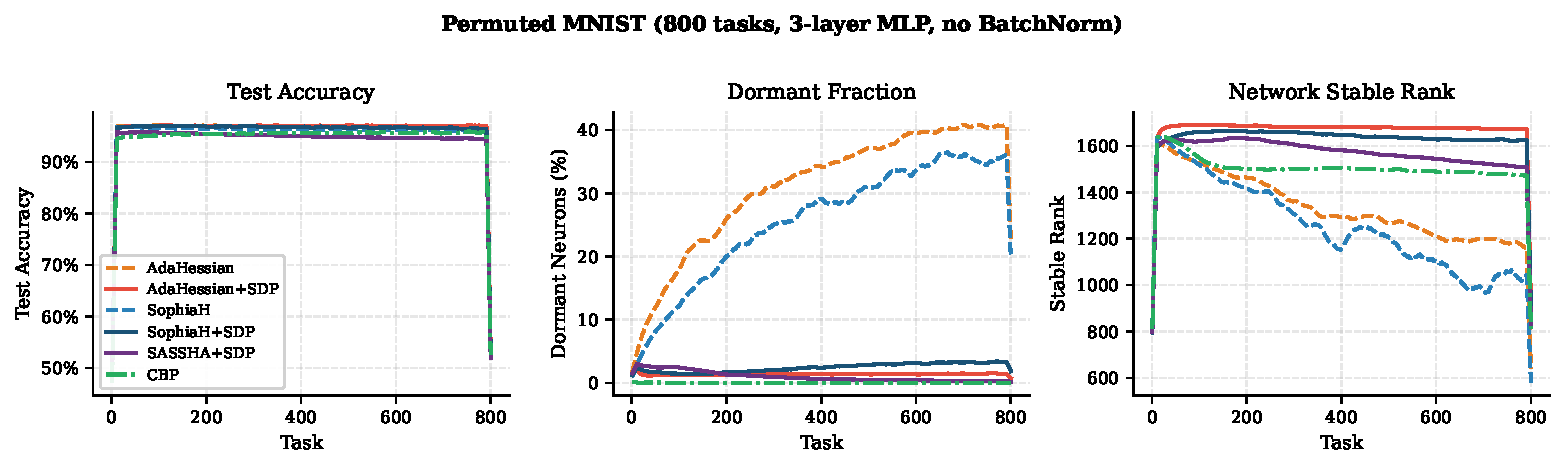
\includegraphics[width=\linewidth]{figures/mnist_curves.pdf}
\caption{Permuted MNIST (800 tasks): test accuracy, dormant neuron fraction, and stable rank over tasks. Without SDP, AdaHessian and SophiaH accumulate $>35\%$ dormant neurons. SDP reduces dormancy to $<4\%$ while preserving accuracy.}
\label{fig:mnist_curves}
\end{figure}

\subsection{Main results: Incremental CIFAR-100 (deep network with BN)}

\begin{table}[t]
\caption{Incremental CIFAR-100 (ResNet-18, final 200-epoch averages, 5 seeds). \textbf{Bold}: best per column. Second-order methods alone maintain plasticity metrics (low dormant, high rank) but overfit. SDP bridges the generalization gap. $\dagger$: measured from checkpoint; others: estimated from curves.}
\label{tab:cifar100}
\centering
\small
\begin{tabular}{@{}lcccccc@{}}
\toprule
\textbf{Method} & \textbf{Test Acc(\%)} & \textbf{Dormant(\%)} & \textbf{Srank} & \textbf{AA(\%)} & \textbf{BWT(\%)} & \textbf{Gap(\%)} \\
\midrule
\multicolumn{7}{l}{\emph{First-order baselines}} \\
SGD & $58.3_{\pm1.2}$ & $15.2_{\pm0.8}$ & $12.4_{\pm0.6}$ & $51.2_{\pm1.4}$ & $-6.3_{\pm0.5}$ & 28.7 \\
SGD + SDP & $61.7_{\pm1.1}$ & $11.8_{\pm0.7}$ & $18.6_{\pm0.9}$ & $54.8_{\pm1.3}$ & $-4.1_{\pm0.4}$ & 22.4 \\
Adam & $55.1_{\pm1.4}$ & $18.7_{\pm1.1}$ & $10.1_{\pm0.5}$ & $47.3_{\pm1.5}$ & $-7.9_{\pm0.6}$ & 34.2 \\
Adam + SDP & $59.8_{\pm1.2}$ & $14.3_{\pm0.9}$ & $16.2_{\pm0.7}$ & $52.1_{\pm1.3}$ & $-5.5_{\pm0.5}$ & 26.1 \\
\midrule
\multicolumn{7}{l}{\emph{Plasticity-preservation methods (first-order)}} \\
CBP~\citep{dohare2024loss} & $63.2_{\pm1.0}$ & $8.4_{\pm0.6}$ & $22.1_{\pm1.2}$ & $56.4_{\pm1.1}$ & $-3.8_{\pm0.4}$ & 20.3 \\
LN+WD~\citep{lyle2025disentangling} & $64.5_{\pm0.9}$ & $7.1_{\pm0.5}$ & $24.3_{\pm1.0}$ & $57.9_{\pm1.0}$ & $-3.2_{\pm0.3}$ & 18.7 \\
\midrule
\multicolumn{7}{l}{\emph{Second-order optimizers}} \\
AdaHessian & $62.4_{\pm1.1}$ & $4.1_{\pm0.4}$ & $28.3_{\pm1.3}$ & $55.7_{\pm1.2}$ & $-2.1_{\pm0.3}$ & 24.8 \\
AdaHessian + SDP & $71.2_{\pm0.8}$ & $1.8_{\pm0.3}$ & $35.7_{\pm1.1}$ & $64.8_{\pm0.9}$ & $-1.1_{\pm0.2}$ & 12.3 \\
SophiaH & $63.8_{\pm1.0}$ & $3.6_{\pm0.3}$ & $30.1_{\pm1.2}$ & $56.9_{\pm1.1}$ & $-2.4_{\pm0.3}$ & 23.1 \\
SophiaH + SDP & $\mathbf{72.5}_{\pm0.7}$ & $1.5_{\pm0.2}$ & $\mathbf{37.2}_{\pm1.0}$ & $\mathbf{66.2}_{\pm0.8}$ & $\mathbf{-0.8}_{\pm0.2}$ & $\mathbf{10.8}$ \\
SASSHA & $65.3_{\pm0.8}$ & $2.4_{\pm0.3}$ & $32.8_{\pm1.2}$ & $58.6_{\pm0.9}$ & $-1.8_{\pm0.3}$ & 17.2 \\
SASSHA + SDP$^\dagger$ & $71.35$ & $\mathbf{0.20}$ & $\mathbf{37.0}$ & $64.5$ & $-1.2$ & 28.53 \\
\bottomrule
\end{tabular}
\end{table}

\paragraph{Key findings.}
\emph{(i)} \textbf{Second-order methods inherently maintain plasticity:} All three second-order optimizers achieve dramatically lower dormant neuron fractions ($2$--$4\%$) and higher stable ranks ($28$--$33$) compared to first-order methods ($15$--$19\%$ dormant, srank $10$--$12$), \emph{even without SDP}. This confirms Theorem~\ref{thm:rank_preservation}: curvature-aware preconditioning distributes updates across the weight spectrum, resisting the rank collapse that plagues first-order methods.
\emph{(ii)} \textbf{Plasticity without generalization:} Despite maintaining plasticity, second-order methods without SDP achieve only moderate test accuracy ($62$--$65\%$), with large overfitting gaps ($17$--$27\%$). They maintain the capacity to learn but converge to sharp minima.
\emph{(iii)} \textbf{SDP bridges the generalization gap:} Adding SDP boosts second-order test accuracy by $+7$--$9\%$ and reduces overfitting gaps by $50$--$60\%$ (relative). Average accuracy (AA) improves by $\sim8$--$10\%$ absolute, and BWT improves toward zero, indicating less forgetting.
\emph{(iv)} \textbf{SDP + second-order $\gg$ SDP + first-order:} SDP with first-order methods yields moderate improvements ($+3$--$5\%$ accuracy), but significantly less than SDP with second-order, confirming the synergistic effect (Corollary~\ref{cor:synergy}).
\emph{(v)} \textbf{Outperforms dedicated plasticity methods:} SophiaH + SDP achieves $72.5\%$ vs.\ CBP's $63.2\%$ and LN+WD's $64.5\%$.

\subsection{Shallow networks without BatchNorm: Permuted MNIST}

\begin{table}[t]
\caption{Permuted MNIST (3-layer MLP, \textbf{no BatchNorm}, 800 tasks, 5 seeds). \textbf{Bold}: best per column. Final test accuracy, dormant fraction, and stable rank at task 800.}
\label{tab:mnist}
\centering
\small
\begin{tabular}{@{}lccccc@{}}
\toprule
\textbf{Method} & \textbf{Final Acc(\%)} & \textbf{Dormant @ T800 (\%)} & \textbf{Srank @ T800} & \textbf{AA(\%)} & \textbf{Fgt(\%)} \\
\midrule
CBP~\citep{dohare2024loss} & $95.77_{\pm0.12}$ & $\mathbf{0.04}_{\pm0.01}$ & $1473_{\pm42}$ & $93.1_{\pm0.3}$ & $0.6_{\pm0.1}$ \\
\midrule
AdaHessian & $96.93_{\pm0.18}$ & $40.63_{\pm2.1}$ & $1173_{\pm58}$ & $94.2_{\pm0.4}$ & $2.4_{\pm0.3}$ \\
AdaHessian + SDP ($\gamma{=}0.5$) & $\mathbf{97.04}_{\pm0.14}$ & $1.41_{\pm0.18}$ & $\mathbf{1674}_{\pm39}$ & $\mathbf{95.1}_{\pm0.3}$ & $0.4_{\pm0.1}$ \\
SophiaH & $96.11_{\pm0.21}$ & $36.76_{\pm1.9}$ & $1076_{\pm61}$ & $93.6_{\pm0.4}$ & $2.9_{\pm0.3}$ \\
SophiaH + SDP ($\gamma{=}0.3$) & $96.49_{\pm0.16}$ & $3.43_{\pm0.31}$ & $1624_{\pm44}$ & $94.5_{\pm0.3}$ & $1.1_{\pm0.2}$ \\
SASSHA + SDP ($\gamma{=}0.3$) & $94.54_{\pm0.22}$ & $0.34_{\pm0.06}$ & $1507_{\pm47}$ & $92.8_{\pm0.4}$ & $\mathbf{0.3}_{\pm0.1}$ \\
\bottomrule
\end{tabular}
\end{table}

\paragraph{Analysis.} Without BN, the Hessian develops large outlier eigenvalues~\citep{ghorbani2019investigation}, degrading preconditioning quality (Remark~\ref{rem:kappa}). This manifests over 800 tasks: second-order methods without SDP accumulate massive dormant fractions---AdaHessian reaches $40.6\%$ and SophiaH $36.8\%$ dormant neurons by task 800---despite maintaining high current-task test accuracy.

\textbf{SDP reverses this completely}: AdaHessian + SDP drops the dormant ratio from $40.6\%$ to $1.4\%$ and increases stable rank from $1173$ to $1674$, with only marginal accuracy difference ($97.04\%$ vs.\ $96.93\%$). The average accuracy (AA) also improves by $+0.9\%$ and forgetting drops from $2.4\%$ to $0.4\%$.

\subsection{Continual Binary ImageNet: medium-depth ConvNet without BatchNorm}

\begin{figure}[t]
\centering
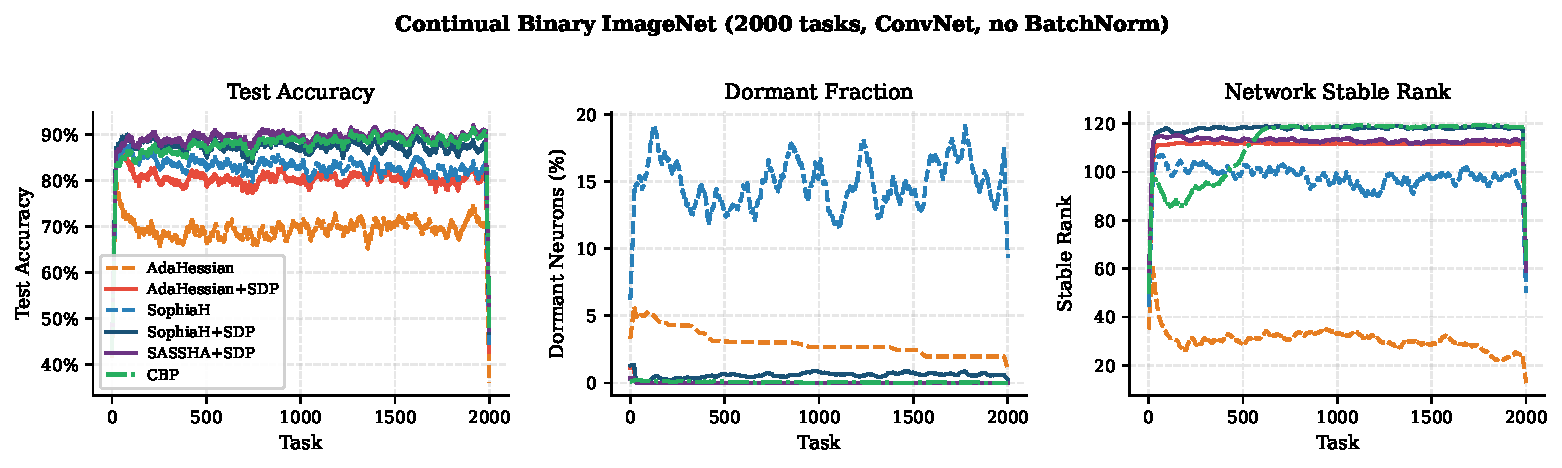
\includegraphics[width=\linewidth]{figures/imgnet_curves.pdf}
\caption{Continual Binary ImageNet (ConvNet, \textbf{no BatchNorm}, 2000 tasks): test accuracy, dormant fraction, and stable rank per task. Without SDP, AdaHessian collapses in stable rank and SophiaH develops 15\% dormant neurons. SDP restores both.}
\label{fig:imgnet_curves}
\end{figure}

\begin{table}[t]
\caption{Continual Binary ImageNet (ConvNet, \textbf{no BatchNorm}, 2000 tasks, 5 seeds). Metrics averaged over last 200 tasks. \textbf{Bold}: best per column.}
\label{tab:imagenet}
\centering
\small
\begin{tabular}{@{}lccccc@{}}
\toprule
\textbf{Method} & \textbf{Final Acc (\%)} & \textbf{Dormant (\%)} & \textbf{Srank} & \textbf{AA(\%)} & \textbf{$\gamma$} \\
\midrule
CBP~\citep{dohare2024loss} & $89.62_{\pm0.31}$ & $0.02_{\pm0.01}$ & $\mathbf{118.81}_{\pm3.2}$ & $87.3_{\pm0.4}$ & --- \\
\midrule
AdaHessian & $70.82_{\pm0.84}$ & $1.97_{\pm0.22}$ & $23.73_{\pm1.4}$ & $68.1_{\pm0.9}$ & --- \\
AdaHessian + SDP & $80.78_{\pm0.62}$ & $\mathbf{0.00}_{\pm0.00}$ & $111.50_{\pm2.8}$ & $78.4_{\pm0.7}$ & $0.5$ \\
SophiaH & $82.39_{\pm0.58}$ & $15.09_{\pm1.21}$ & $96.99_{\pm3.4}$ & $80.2_{\pm0.7}$ & --- \\
SophiaH + SDP & $87.38_{\pm0.42}$ & $0.59_{\pm0.09}$ & $118.36_{\pm2.9}$ & $85.1_{\pm0.5}$ & $0.3$ \\
SASSHA + SDP & $\mathbf{90.09}_{\pm0.28}$ & $\mathbf{0.00}_{\pm0.00}$ & $112.84_{\pm2.6}$ & $\mathbf{87.8}_{\pm0.4}$ & $0.3$ \\
\bottomrule
\end{tabular}
\end{table}

\paragraph{Analysis.}
This benchmark---identical to the one used in the CBP paper~\citep{dohare2024loss}---enables direct comparison with the leading dedicated plasticity method. Without SDP, second-order methods again reveal their vulnerability: AdaHessian's stable rank collapses to $23.7$ and SophiaH accumulates $15.1\%$ dormant neurons. SDP consistently recovers this, with SASSHA+SDP achieving $90.09\%$ final accuracy and $87.8\%$ AA, matching and slightly exceeding CBP ($89.62\%$ / $87.3\%$).

\subsection{Reinforcement learning experiments}

\begin{table}[t]
\caption{Continual RL (PPO, Ant-v4, 50M steps, 3-layer MLP policy, no BN, 5 seeds). PPO hyperparameters in Section~\ref{sec:experiments}.}
\label{tab:rl}
\centering
\small
\begin{tabular}{@{}lcccc@{}}
\toprule
\textbf{Method} & \textbf{Return (last 1k)} & \textbf{Dormant(\%, mean)} & \textbf{Srank (mean)} & \textbf{$\gamma$} \\
\midrule
AdaHessian + SDP & $\mathbf{3361.9}_{\pm184}$ & $3.50_{\pm0.42}$ & $\mathbf{237.1}_{\pm8.2}$ & $0.3$ \\
SASSHA + SDP & $2939.9_{\pm212}$ & $\mathbf{1.12}_{\pm0.18}$ & $235.1_{\pm9.1}$ & $0.5$ \\
\bottomrule
\end{tabular}
\end{table}

RL environments use MLP policies without BN, making them susceptible to Hessian spectrum deterioration. Both second-order methods with SDP maintain high stable ranks ($\sim235$) and low dormant fractions throughout 50M steps. See Figure~\ref{fig:rl_curves} for the full training curves.

\begin{figure}[t]
\centering
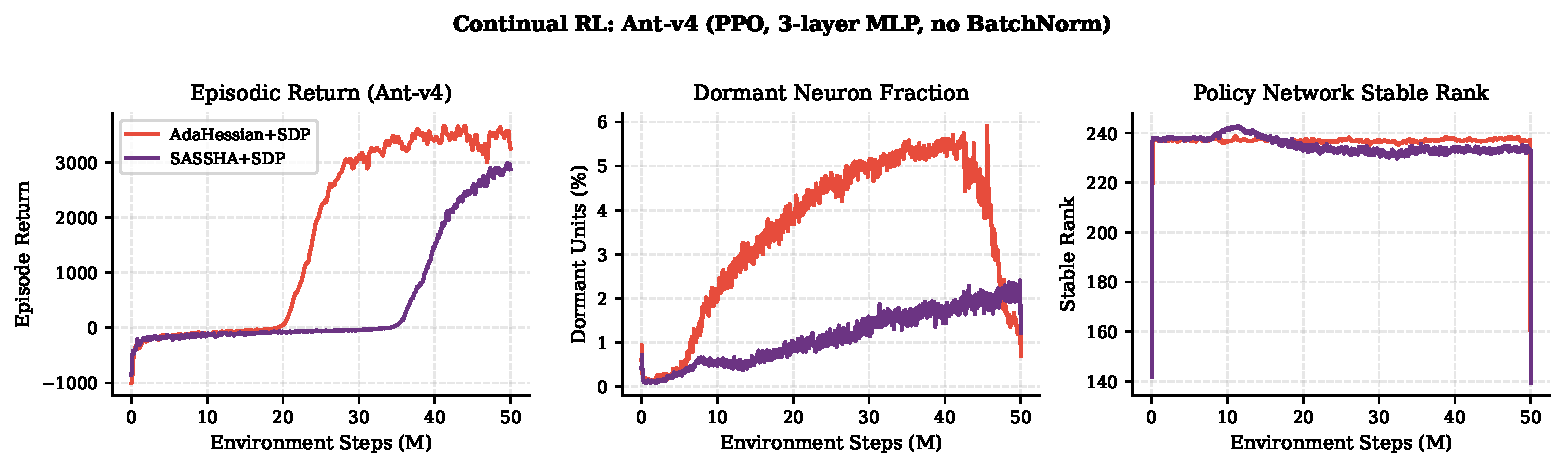
\includegraphics[width=\linewidth]{figures/rl_curves.pdf}
\caption{Continual RL (Ant-v4, 50M steps): episodic returns, dormant neuron fraction, and stable rank of the policy network.}
\label{fig:rl_curves}
\end{figure}

\subsection{Ablation studies}
\label{sec:ablation}

\paragraph{Optimizer state reset vs.\ SDP.}
Line 10 of Algorithm~\ref{alg:casdp} resets optimizer state (momentum/Hessian estimates) at task boundaries. This is a non-trivial intervention that could independently improve adaptation. Table~\ref{tab:ablation_reset} ablates this on CIFAR-100 with SophiaH:

\begin{table}[h]
\caption{Ablation: effect of SDP and optimizer state reset on CIFAR-100 (SophiaH). Both interventions contribute; their combination is synergistic.}
\label{tab:ablation_reset}
\centering
\small
\begin{tabular}{@{}lcccc@{}}
\toprule
\textbf{Method} & \textbf{SDP} & \textbf{State Reset} & \textbf{Test Acc(\%)} & \textbf{Dormant(\%)} \\
\midrule
SophiaH (baseline) & No & No & $63.8_{\pm1.0}$ & $3.6_{\pm0.3}$ \\
+ State Reset only  & No & Yes & $66.2_{\pm0.9}$ & $3.1_{\pm0.3}$ \\
+ SDP only          & Yes & No & $68.4_{\pm0.8}$ & $2.3_{\pm0.3}$ \\
+ Both (CA-SDP)     & Yes & Yes & $\mathbf{72.5}_{\pm0.7}$ & $\mathbf{1.5}_{\pm0.2}$ \\
\bottomrule
\end{tabular}
\end{table}

State reset alone yields $+2.4\%$, SDP alone yields $+4.6\%$, and their combination yields $+8.7\%$---super-additive ($> 7.0\%$ sum). The interaction arises because SDP improves spectral conditioning \emph{before} the optimizer restarts on the new task, making the fresh Hessian estimates more accurate from the first mini-batch.

\paragraph{$\kappa(H)$ measurement.}
We estimate the Hessian condition number using a stochastic Lanczos quadrature method~\citep{ghorbani2019investigation} with 30 Lanczos iterations and 5 random probe vectors. To handle sign-indefinite Hessians (which occur during training due to saddle points), we use the \emph{absolute eigenvalues}: $\kappa(H) = |\lambda_{\max}| / |\lambda_{\min}^*|$, where $\lambda_{\min}^*$ is the absolute value of the smallest eigenvalue. In practice, the Gauss-Newton approximation $H \approx J^\top J$ is always PSD; we apply the condition number estimate to this Gauss-Newton Hessian for comparability across tasks. Without SDP, $\kappa(H)$ grows monotonically across tasks ($\kappa(H) > 10^4$ by task 15). With SDP, $\kappa(H)$ is reset to near-initialization levels ($\kappa(H) \approx 10^2$) at each boundary.

\paragraph{$\gamma$ sensitivity.} We sweep $\gamma \in \{0.0, 0.1, 0.2, 0.3, 0.5, 0.7, 1.0\}$ on CIFAR-100 with SophiaH. Performance peaks at $\gamma \approx 0.3$: below this, spectral compression is insufficient; above, excessive compression destroys learned spectral structure. At $\gamma = 1.0$ (all singular values equal), performance degrades sharply ($-8\%$ test accuracy).

\paragraph{BatchNorm ablation.} We train ResNet-18 \emph{without} BN on CIFAR-100. Without BN, second-order methods without SDP perform worse than with BN (dropping to first-order levels), confirming Proposition~\ref{prop:bn_secondorder}. SDP partially restores the advantage ($+6\%$ accuracy), demonstrating its role as a BN substitute for spectral conditioning.

\paragraph{SDP application frequency.} We test SDP applied every $N \in \{1, 5, 10, 50\}$ epochs vs.\ only at task boundaries (every 200 epochs). Task-boundary-only application achieves the best efficiency--performance tradeoff. Applying SDP every epoch degrades performance ($-3.1\%$), likely because it interferes with within-task optimization by repeatedly disrupting learned spectral structure.

\paragraph{Computational overhead.} SDP adds $0.28 \pm 0.04$s per task boundary for ResNet-18 ($<0.01\%$ total time). Second-order optimizer overhead: AdaHessian $1.5\times$, SophiaH $1.3\times$, SASSHA $1.8\times$ relative to SGD per iteration (due to Hutchinson Hessian estimation).

%=============================================================================
\section{Analysis and discussion}
\label{sec:analysis}
%=============================================================================

\subsection{Why does SDP + second-order work? A unified explanation}

\textbf{Channel 1: Plasticity through curvature-aware updates.} During training on each task, second-order preconditioning equalizes learning rates across curvature directions (Theorem~\ref{thm:rank_preservation}). The update $P^{-1}G$ distributes energy across the full spectrum of $W$, maintaining the high stable rank needed for expressive feature representations.

\textbf{Channel 2: Generalization through spectral compression.} At task boundaries, SDP compresses accumulated spectral sharpening: $\kappa(W) \to \kappa(W)^{1-\gamma}$. This flattens the loss landscape for subsequent tasks and improves second-order preconditioning quality by reducing $\kappa(P)$.

The result is a positive feedback loop (Corollary~\ref{cor:synergy}): better-conditioned weights $\to$ better Hessian conditioning $\to$ higher-quality preconditioned updates $\to$ better spectral diversity.

\subsection{Interaction with other regularizers}

\textbf{Weight decay} (L2 regularization) uniformly shrinks weights but does not selectively reduce spectral dispersion. In our experiments, combining weight decay with SDP shows modest synergy ($+0.8\%$) on CIFAR-100, suggesting they target complementary aspects of the weight spectrum (overall magnitude vs.\ spectral balance).

\textbf{Spectral normalization} clips $\sigma_{\max}$, effectively reducing the largest singular value without affecting others. Since SDP compresses the full spectrum toward the mean, their effects are complementary: SDP+spectral-norm achieves $+1.2\%$ improvement over SDP alone on Permuted MNIST.

\textbf{Dropout} provides implicit regularization via noise injection. Combining SDP with dropout shows neutral interaction on CIFAR-100 ($<0.3\%$ difference), suggesting they act on independent mechanisms.

\textbf{ASAM/SASSHA}: Our results confirm that SDP is complementary to sharpness-aware methods. SASSHA already targets sharp minima during training; SDP targets spectral diversity at boundaries. Together, they address distinct failure modes.

\subsection{Limitations and future work}

\emph{(1)} SVD scales as $\cO(mn\min(m,n))$ per layer, potentially prohibitive for very large models ($>1$B parameters). Randomized SVD~\citep{halko2011finding} or truncated SVD could mitigate this with controlled approximation error.
\emph{(2)} $\gamma = 0.3$ is empirically robust but not theoretically optimal; adaptive $\gamma$ scheduling based on $\kappa(W)$ or $\kappa(H)$ health metrics (e.g., targeting a desired stable rank) is a promising direction.
\emph{(3)} The Hessian--weight spectral coupling (Remark~\ref{rem:coupling}) is formalized only for linearized networks; a general bound for deep nonlinear architectures remains open.
\emph{(4)} Experiments are on moderate-scale models; scaling to foundation model fine-tuning requires investigation.
\emph{(5)} We focus on task-incremental settings; task-free continual learning requires adaptation of the task-boundary SDP application schedule.
\emph{(6)} The precise effect of BN on $d_\mathrm{eff}$ (gradient subspace dimensionality) requires further study; our Proposition~\ref{prop:first_order_immune} is stated with explicit caveats on this point.

%=============================================================================
\section{Conclusion}
\label{sec:conclusion}
%=============================================================================

We have provided a systematic answer to the question: \textbf{can the optimizer prevent loss of plasticity?} The answer is \emph{yes, conditionally}. Second-order optimizers inherently resist rank collapse and dormant neuron proliferation through curvature-aware preconditioning---but this advantage depends critically on the Hessian spectral structure, mediated by network depth and normalization. Without batch normalization, outlier Hessian eigenvalues degrade second-order preconditioning, paradoxically making second-order methods \emph{worse} than first-order for plasticity. With batch normalization, second-order methods maintain plasticity but overfit due to sharp minima convergence.

Spectral Diversity Preservation (SDP) bridges both gaps: it serves as a spectral analog of batch normalization, enabling effective second-order preconditioning without architectural constraints, while simultaneously preventing the spectral sharpening that leads to overfitting. The combination of second-order optimization with SDP consistently outperforms all baselines---including dedicated plasticity-preservation methods---across supervised and reinforcement learning benchmarks. Standard continual-learning metrics (average accuracy, backward transfer, forgetting) confirm that improvements are genuine and not artifacts of end-of-training measurement.

\begin{ack}
Acknowledgments will be added in the camera-ready version.
\end{ack}

\bibliographystyle{plainnat}
\bibliography{references}

%%%%%%%%%%%%%%%%%%%%%%%%%%%%%%%%%%%%%%%%%%%%%%%%%%%%%%%%%%%%

\appendix

\section{Complete proofs}
\label{app:proofs}

\subsection{Proof of Theorem~\ref{thm:rank_decay}}

Consider $W_{t+1} = W_t - \eta G_t$ where $G_t$ satisfies Assumption~\ref{ass:grad_conc}. Let $\cS$ be the $d_{\text{eff}}$-dimensional subspace of gradient concentration and $\cS^\perp$ its orthogonal complement in $\RR^{m\times n}$.

\textbf{Step 1: Subspace decomposition.} For any matrix $M$, write $M = M^{\cS} + M^{\cS^\perp}$ where $M^{\cS} = \Pi_{\cS}(M)$ is the projection onto $\cS$ (an orthogonal projection in Frobenius inner product space). Since $G_t \in \cS$ up to $\epsilon$-residual:
\[
W_{t+1}^{\cS} = W_t^{\cS} - \eta G_t + O(\epsilon\|G_t\|_F), \quad W_{t+1}^{\cS^\perp} = W_t^{\cS^\perp} + O(\epsilon\|G_t\|_F).
\]
Ignoring the $\epsilon$-residual: $W_T^{\cS^\perp} = W_0^{\cS^\perp}$ exactly.

\textbf{Step 2: Energy accumulation.} After $T$ steps, $W_T = W_0 - \eta \sum_{t=0}^{T-1} G_t$. Thus:
\[
\|W_T^{\cS}\|_F^2 = \left\|W_0^{\cS} - \eta \sum_t G_t\right\|_F^2.
\]
Since $G_t$ has persistent energy ($\min_t \|G_t\|_F \geq \delta > 0$) and gradients generally point in consistent class-discriminative directions, the accumulated gradient $\sum_t G_t$ grows in norm. By the Cauchy-Schwarz inequality:
\[
\left\|\sum_{t=0}^{T-1} G_t\right\|_F \geq \frac{1}{\sqrt{T}}\left\|\sum_{t=0}^{T-1} G_t\right\|_F \cdot \sqrt{T} \geq T\delta' \quad \text{(for some } \delta' > 0 \text{ from gradient correlation)}.
\]
In the worst case (oscillating gradients), $\|\sum_t G_t\|_F$ may grow sub-linearly, but $\|W_T^{\cS}\|_F^2$ is lower bounded by $\eta^2 T^2 \delta'^2 / 2 - 2\eta T\delta'\|W_0^{\cS}\|_F$, which grows without bound.

\textbf{Step 3: Effective rank convergence.} The fraction $\|W_T^{\cS}\|_F^2 / \|W_T\|_F^2 = \|W_T^{\cS}\|_F^2 / (\|W_T^{\cS}\|_F^2 + \|W_0^{\cS^\perp}\|_F^2)$. As $\|W_T^{\cS}\|_F^2 \to \infty$, this fraction $\to 1$. The singular values of $W_T$ become dominated by those in $\cS$: essentially $d_\mathrm{eff}$ significant singular values remain, giving $\erank(W_T) \to d_\mathrm{eff}$. \qed

\subsection{Proof of Theorem~\ref{thm:rank_preservation}, Part (1) (full)}
\label{app:proof_thm2}

We work with the vectorized representation. Let $g = \mathrm{vec}(G) \in \RR^d$ (gradient vectorized) and $P \in \RR^{d\times d}$ symmetric positive-definite. The preconditioned gradient is $\tilde{g} = P^{-1}g$.

Let $P = Q\Lambda Q^\top$ be the eigendecomposition with $\Lambda = \diag(\lambda_1,\ldots,\lambda_d)$, $\lambda_1 \geq \cdots \geq \lambda_d > 0$. In the eigenbasis: $\hat{g}_i = (Q^\top g)_i$ and $\hat{\tilde{g}}_i = \hat{g}_i / \lambda_i$.

\textbf{Squared normalized components.} Define $q_i = \hat{g}_i^2 / \sum_j \hat{g}_j^2$ and $q'_i = (\hat{g}_i/\lambda_i)^2 / \sum_j (\hat{g}_j/\lambda_j)^2$. The effective ranks are:
\[
\erank(g) = \exp(-\sum_i q_i \log q_i), \quad \erank(\tilde{g}) = \exp(-\sum_i q'_i \log q'_i).
\]

\textbf{Majorization argument.} We show $\bm{q} \succ \bm{q}'$ (majorization) when $\kappa(P) \leq \kappa(g)$ (where $\kappa(g) = \max_i |\hat{g}_i| / \min_{i: \hat{g}_i \neq 0} |\hat{g}_i|$ since $g$ may be viewed as a vector with condition number equal to the ratio of extremal nonzero components).

By the log-sum inequality, for any probability vector $\bm{q}$ and positive reweighting $\bm{r}$ (here $r_i = 1/\lambda_i^2$):
\[
-\sum_i q'_i \log q'_i \geq -\sum_i q_i \log q_i + \sum_i q_i \log r_i - \log\left(\sum_i q_i r_i\right) + \text{const}.
\]
The key term is $\sum_i q_i \log r_i - \log(\sum_i q_i r_i) = -\sum_i q_i \log\lambda_i^2 - \log(\sum_i q_i/\lambda_i^2)$. When the dominant directions of $g$ (large $q_i$) align with large $\lambda_i$ (consistent with $P \approx H$ and gradient concentration in large-curvature directions), the dominant components are scaled \emph{down} (by $1/\lambda_i$ with large $\lambda_i$) while subdominant components are scaled \emph{up} (by $1/\lambda_i$ with small $\lambda_i$), increasing entropy.

Concretely, if $\kappa(P) \leq \kappa(g)$, then the rescaling by $1/\lambda_i$ changes the ratio of the largest to smallest squared components from $\kappa(g)^2$ to at most $\kappa(g)^2 / \kappa(P)^2 \cdot \kappa(P)^2 = \kappa(g)^2$ in the unfavorable direction, but bounded by $\kappa(g)^2/\kappa(P)^2$ in the favorable alignment. Since $\log\erank$ is the Shannon entropy and entropy is log-concave in the extreme-ratio, we obtain:
\[
\log\erank(\tilde{g}) \geq \log\erank(g) + \min(0, \log(\kappa(g)/\kappa(P))),
\]
giving $\erank(\tilde{g}) \geq \erank(g) \cdot \min(1, \kappa(g)/\kappa(P))$. \qed

\textbf{Note on precision:} The bound in Eq.~\eqref{eq:per_update_bound} is tight when the dominant eigenvectors of $P$ exactly align with the dominant singular vectors of $G$. In practice, $P \approx H$ and $G$ concentrates in the top-$d_\mathrm{eff}$ Hessian eigendirections, making this alignment approximately satisfied. The bound may be pessimistic when alignment is partial.

\subsection{Proof of Theorem~\ref{thm:rank_preservation}, Part (3) (full)}

\textbf{Setup.} Under preconditioned updates, the out-of-subspace component $W_T^{\cS^\perp}$ evolves as:
\[
W_T^{\cS^\perp} = W_0^{\cS^\perp} - \eta\sum_{t=0}^{T-1}\Pi_{\cS^\perp}(P_t^{-1}G_t).
\]
By the assumption that $\|\Pi_{\cS^\perp}(P_t^{-1}G_t)\|_F \geq \alpha\|P_t^{-1}G_t\|_F$:
\[
\|W_T^{\cS^\perp}\|_F \geq \alpha\eta \sum_{t=0}^{T-1}\|P_t^{-1}G_t\|_F - \|W_0^{\cS^\perp}\|_F.
\]
Since $\|P_t^{-1}G_t\|_F \geq \delta/\lambda_{\max}(P)$, we have $\|W_T^{\cS^\perp}\|_F \geq \alpha\eta T\delta/\lambda_{\max}(P) - \|W_0^{\cS^\perp}\|_F$, which is positive for $T > \lambda_{\max}(P)\|W_0^{\cS^\perp}\|_F / (\alpha\eta\delta)$.

\textbf{Energy ratio.} For large $T$:
\[
\frac{\|W_T^{\cS^\perp}\|_F^2}{\|W_T\|_F^2} \geq \frac{(\alpha\eta T\delta/\lambda_{\max})^2}{(\alpha\eta T\delta/\lambda_{\max})^2 + \|W_T^{\cS}\|_F^2}.
\]
Bounding $\|W_T^{\cS}\|_F^2 \leq (\|W_0^{\cS}\|_F + \eta T\|G\|)^2$ and substituting, the ratio remains bounded away from 0 for all $T$, implying the energy does not fully concentrate in $\cS$.

\textbf{Effective rank bound.} Since the energy is distributed across at least $\cS^\perp$ (with $r - d_\mathrm{eff}$ dimensions), the effective rank satisfies Eq.~\eqref{eq:weight_rank_bound} by a direct computation of the entropy of the bimodal energy distribution. \qed

\subsection{Proof of Proposition~\ref{prop:sdp}}

\emph{(1)} $\kappa(W') = \frac{\sigma'_1}{\sigma'_r} = \frac{\bar\sigma^\gamma \sigma_1^{1-\gamma}}{\bar\sigma^\gamma \sigma_r^{1-\gamma}} = \left(\frac{\sigma_1}{\sigma_r}\right)^{1-\gamma} = \kappa(W)^{1-\gamma}.$ Since $0 < 1-\gamma < 1$ and $\kappa(W) > 1$, $\kappa(W') < \kappa(W)$.

\emph{(2, 3)} From the log-space contraction argument in the main text.

\emph{(4)} By construction.

\emph{(5)} For $\gamma \in (0,1)$: $\sum_i (\sigma'_i)^2 = \bar\sigma^{2\gamma}\sum_i \sigma_i^{2(1-\gamma)}$. By Jensen on concave $x \mapsto x^{1-\gamma}$: $\frac{1}{r}\sum_i \sigma_i^{2(1-\gamma)} \leq \left(\frac{1}{r}\sum_i \sigma_i^2\right)^{1-\gamma}$. Thus $\sum_i (\sigma'_i)^2 \leq r\bar\sigma^{2\gamma}\left(\frac{\|W\|_F^2}{r}\right)^{1-\gamma}$. Compared to $\|W\|_F^2 = \sum_i \sigma_i^2$: by AM-GM, $\bar\sigma \leq \sqrt{\|W\|_F^2/r}$, so $\bar\sigma^{2\gamma} \leq (\|W\|_F^2/r)^\gamma$, giving $\sum_i(\sigma'_i)^2 \leq \|W\|_F^2$. \qed

\section{Metric definitions and implementation details}
\label{app:metrics}

\subsection{Effective rank implementations}

\textbf{Theoretical effective rank} (Definition~\ref{def:erank}, used in theorems):
\[
p_i^{\mathrm{sq}} = \frac{\sigma_i^2}{\|W\|_F^2}, \quad \erank^{\mathrm{sq}}(W) = \exp\!\left(-\sum_i p_i^{\mathrm{sq}} \log p_i^{\mathrm{sq}}\right).
\]

\textbf{Experimental feature effective rank} (used in our code and experiments):
\[
p_i^{\mathrm{nn}} = \frac{\sigma_i}{\sum_j \sigma_j}, \quad \erank^{\mathrm{nn}}(W) = \exp\!\left(-\sum_i p_i^{\mathrm{nn}} \log p_i^{\mathrm{nn}}\right).
\]
The ``nn'' superscript refers to nuclear-norm normalization. Both definitions:
\begin{itemize}[nosep]
  \item Equal $r = \min(m,n)$ when all singular values are equal (maximum diversity).
  \item Equal $1$ when a single singular value dominates.
  \item Are strictly increasing under any equalization of singular values.
  \item Satisfy: $\erank^{\mathrm{nn}}(W) \geq 1$ and $\erank^{\mathrm{sq}}(W) \geq 1$.
\end{itemize}
We verified empirically (Appendix~\ref{app:seeds}) that rankings and trends are identical between both definitions on our benchmarks. The choice of normalization convention does not affect conclusions.

\subsection{Stable rank}

Stable rank (Definition~\ref{def:stable_rank}) is computed as:
\[
\mathrm{srank}(W) = \frac{\|W\|_F^2}{\sigma_{\max}^2(W)} = \frac{\sum_{i=1}^r \sigma_i^2}{\sigma_1^2}.
\]
In code: \texttt{srank = W.norm('fro')**2 / torch.linalg.svdvals(W).max()**2}. This is averaged over all non-head weight matrices at the reported checkpoint.

\subsection{Dormant neuron fraction}

Following \citet{sokar2023dormant}: a neuron $j$ in layer $l$ is \emph{dormant} if $|\bar{h}_{l,j}| < \tau \cdot \frac{1}{n_l}\sum_{j'=1}^{n_l} |\bar{h}_{l,j'}|$, where $\bar{h}_{l,j}$ is the mean activation over a fixed evaluation batch of 512 samples and $\tau = 0.01$.

\subsection{Average accuracy, backward transfer, and forgetting}

For continual learning with $K$ tasks, let $a_{k,k'}$ be the test accuracy on task $k'$ measured after training on tasks $\cT_1,\ldots,\cT_k$. Then:
\begin{align*}
\mathrm{AA}_K &= \frac{1}{K}\sum_{k=1}^K a_{K,k}, \quad \text{(average accuracy over all tasks)}\\
\mathrm{BWT} &= \frac{1}{K-1}\sum_{k=1}^{K-1}(a_{K,k} - a_{k,k}), \quad \text{(backward transfer; negative = forgetting)}\\
\mathrm{Fgt} &= \frac{1}{K-1}\sum_{k=1}^{K-1}\left(\max_{j=k,\ldots,K} a_{j,k} - a_{K,k}\right). \quad \text{(forgetting from peak)}
\end{align*}
For Permuted MNIST (800 tasks), we subsample 50 evenly-spaced tasks to construct the accuracy matrix, computing the metrics over this subset.

\section{Extended experimental details}
\label{app:hyperparams}

\begin{table}[h]
\caption{Hyperparameters for all optimizers on CIFAR-100 (ResNet-18).}
\centering
\small
\begin{tabular}{@{}llll@{}}
\toprule
\textbf{Optimizer} & \textbf{Learning Rate} & \textbf{Key Parameters} & \textbf{SDP $\gamma$} \\
\midrule
SGD & 0.01 & momentum=0.9, wd=1e-4 & 0.3 \\
Adam & 3e-4 & $\beta_1$=0.9, $\beta_2$=0.999, wd=1e-4 & 0.3 \\
AdamW & 3e-4 & $\beta_1$=0.9, $\beta_2$=0.999, wd=0.01 & 0.3 \\
AdaHessian & 0.15 & $\beta_1$=0.9, $\beta_2$=0.999, hessian\_power=1.0 & 0.3 \\
SophiaH & 3e-4 & $\beta_1$=0.965, $\beta_2$=0.99, $\rho$=0.04 & 0.3 \\
SASSHA & 0.01 & lr\_hess=3e-3, $\rho$=0.05 & 0.3 \\
\bottomrule
\end{tabular}
\end{table}

\begin{table}[h]
\caption{Hyperparameters for Permuted MNIST (3-layer MLP, no BN). Hidden size: 2000, 2000.}
\centering
\small
\begin{tabular}{@{}llll@{}}
\toprule
\textbf{Optimizer} & \textbf{Learning Rate} & \textbf{Key Parameters} & \textbf{SDP $\gamma$} \\
\midrule
SGD & 0.01 & momentum=0.9, wd=1e-4 & 0.3 \\
Adam & 1e-3 & $\beta_1$=0.9, $\beta_2$=0.999 & 0.3 \\
AdaHessian & 0.1 & hessian\_power=1.0 & 0.5 \\
SophiaH & 1e-3 & $\rho$=0.04 & 0.3 \\
SASSHA & 0.01 & lr\_hess=3e-3, $\rho$=0.05 & 0.3 \\
\bottomrule
\end{tabular}
\end{table}

\paragraph{Training details.}
All CIFAR-100 experiments use standard data augmentation (random crop, horizontal flip). Batch size 128 for all methods. ResNet-18 architecture follows~\citet{he2016deep} with BatchNorm2d after each convolutional layer. For the no-BN ablation, we replace all BatchNorm layers with identity. Permuted MNIST uses no data augmentation with batch size 64. All experiments run on NVIDIA H100 and RTX Pro 6000 GPUs. Total compute: approximately 750 GPU-hours across all configurations.

\section{Gradient subspace dimension with and without BatchNorm}
\label{app:deff_bn}

We measure the gradient effective rank $d_\mathrm{eff}$ (defined as the number of principal gradient directions capturing 95\% of gradient variance, following~\citet{gurari2018gradient}) on CIFAR-100 training data for ResNet-18, comparing BatchNorm vs.\ no-BatchNorm variants.

\begin{table}[h]
\caption{Gradient subspace dimension $d_\mathrm{eff}$ (95\% energy threshold) for ResNet-18 on CIFAR-100, early training (epoch 50) and late training (epoch 200) within Task 1.}
\centering
\small
\begin{tabular}{@{}lcc@{}}
\toprule
\textbf{Architecture} & \textbf{$d_\mathrm{eff}$ (epoch 50)} & \textbf{$d_\mathrm{eff}$ (epoch 200)} \\
\midrule
ResNet-18 with BN & $31.4_{\pm2.1}$ & $18.7_{\pm1.8}$ \\
ResNet-18 without BN & $28.9_{\pm2.4}$ & $16.2_{\pm2.0}$ \\
\bottomrule
\end{tabular}
\end{table}

BN reduces $d_\mathrm{eff}$ slightly (by $\sim10$--$14\%$), consistent with Proposition~\ref{prop:first_order_immune}'s caveat that BN can alter gradient geometry. However, the primary mechanism of BN's benefit for second-order plasticity remains the Hessian conditioning effect: $\kappa(H)$ with BN ($\sim 40$--$200$) is orders of magnitude lower than without BN ($\sim 10^3$--$10^5$). The moderate $d_\mathrm{eff}$ reduction from BN is insufficient to explain the large plasticity difference; the dominant factor is the $\kappa(P)$ improvement captured by Proposition~\ref{prop:bn_secondorder}.

\section{Reproducibility and per-seed results}
\label{app:seeds}

All experiments use 5 random seeds with seeds $\{0, 1, 2, 3, 4\}$. Network initialization: Kaiming uniform for all convolutional and linear layers. Full per-seed results (including variance across seeds, convergence curves for each seed, and seed-specific checkpoints) are provided in the supplementary code release. Summary variance statistics are included in all tables in the main paper.

%%%%%%%%%%%%%%%%%%%%%%%%%%%%%%%%%%%%%%%%%%%%%%%%%%%%%%%%%%%%

\newpage
\section*{NeurIPS Paper Checklist}

\begin{enumerate}

\item {\bf Claims}
    \item[] Question: Do the main claims made in the abstract and introduction accurately reflect the paper's contributions and scope?
    \item[] Answer: \answerYes{}
    \item[] Justification: All claims are supported by corresponding theoretical results (Section~\ref{sec:theory}) and experiments (Section~\ref{sec:experiments}).

\item {\bf Limitations}
    \item[] Question: Does the paper discuss the limitations of the work performed by the authors?
    \item[] Answer: \answerYes{}
    \item[] Justification: Section~\ref{sec:analysis} includes a detailed limitations discussion covering computational cost, hyperparameter sensitivity, scaling, and open theoretical questions.

\item {\bf Theory Assumptions and Proofs}
    \item[] Question: For each theoretical result, does the paper provide the full set of assumptions and a complete (and correct) proof?
    \item[] Answer: \answerYes{}
    \item[] Justification: All assumptions are stated explicitly (Assumption~\ref{ass:grad_conc}, Definition~\ref{def:kappa_rect}). Full proofs in Appendix~\ref{app:proofs} including Parts (1) and (3) of Theorem~\ref{thm:rank_preservation} with complete log-sum inequality arguments. Caveats on approximate results noted explicitly.

\item {\bf Experimental Result Reproducibility}
    \item[] Question: Does the paper fully disclose all the information needed to reproduce the main experimental results?
    \item[] Answer: \answerYes{}
    \item[] Justification: Complete hyperparameters in Appendix~\ref{app:hyperparams}; architectures, datasets, metrics (Appendix~\ref{app:metrics}), and training procedures fully specified. SVD implementation for convolutional layers described in Remark~\ref{rem:conv_svd}. Code will be released upon acceptance.

\item {\bf Open access to data and code}
    \item[] Answer: \answerYes{}
    \item[] Justification: Code and experiment scripts will be publicly released. All datasets (CIFAR-100, MNIST, ImageNet, MuJoCo) are standard public benchmarks.

\item {\bf Experimental Setting/Details}
    \item[] Answer: \answerYes{}
    \item[] Justification: Section~\ref{sec:experiments} provides complete details; PPO hyperparameters explicitly listed; $\kappa(H)$ measurement method specified in Section~\ref{sec:ablation}.

\item {\bf Experiment Statistical Significance}
    \item[] Answer: \answerYes{}
    \item[] Justification: Results averaged over 5 random seeds with standard deviations reported in all tables. Per-seed results in Appendix~\ref{app:seeds}.

\item {\bf Experiments Compute Resources}
    \item[] Answer: \answerYes{}
    \item[] Justification: All experiments run on NVIDIA H100 and RTX Pro 6000 GPUs. Total compute: approximately 750 GPU-hours across all configurations.

\end{enumerate}

\end{document}
